%\documentclass[tikz,svgnames,border={0 2}]{standalone}
\renewcommand\vec[1]{\boldsymbol{#1}}

%\begin{document}
\begin{tikzpicture}[
    box/.style={rectangle,draw,fill=DarkGray!20,node distance=1cm,text width=15em,text centered,rounded corners,minimum height=2em,thick},
    arrow/.style={draw,-latex',thick},
  ]

  \node [box] (potential) {$v_{\text{ext},s}(\vec r)=v_\text{H}(\vec r) + v_\text{xc}(\vec r) + v_\text{ext}(\vec r)$};
  \node [box,below=0.5 of potential] (hamiltonian) {$\hat{H}_{KS}=-\frac{\hbar^2}{2m}\vec{\nabla}^2 + v_{\text{ext},s}(\vec r)$};
  \node [box,below=0.5 of hamiltonian] (se) {$\hat{H}_{KS} \phi_i(\vec r)= E_i \phi_i(\vec r)$};
  \node [box,below=0.5 of se] (density) {$\rho(\vec r)=\sum_{i=1}^n f_i\,|\phi_i(\vec r_i)|^2$};
  \node [box,below=0.5 of density] (criterion) {Convergence criterion satisfied?};

%%%%%% ------------ 定义 虚线方框转角 -----------------  %%%%%%
  \path
  (potential.north west) ++(-1em,1em) coordinate (potential fit)
  (criterion.south east) ++(1em,-1em) coordinate (criterion fit);

  \node [box,above=1.5 of potential, fill=orange!30, text width=20em] (initial) {Supply initial density guess $\rho_\text{ini}(\vec r)$ to Kohn Sham equations};
  \node [box,below=1.5 of criterion, fill=blue!30, text width=20em] (energy) {Use $\rho_\text{fin}(\vec r)$ to minimize total energy functional $E_{V_\text{ext}}[\rho]=T_{e,s}[\phi_i\{\rho\}] + V_{ee,H}[\rho] + E_{xc}[\rho] + V_{eI}[\rho]$};

  \path [arrow] (initial) -- (potential);
  \path [arrow] (potential) -- (hamiltonian);
  \path [arrow] (hamiltonian) -- (se);
  \path [arrow] (se) -- (density);
  \path [arrow] (density) -- (criterion);

%%%%%% ------------ 绘制 虚线方框 -----------------  %%%%%%
  \node [rectangle,draw,dashed,inner sep=1em,fit=(potential fit) (criterion fit)] (enclosure) {};
  \node [above=-0.8em of enclosure,anchor=south,draw,outer sep=0pt,fill=white] (enclosure label) {\Large\textbf{Kohn-Sham method}};

  \path [arrow] (criterion) -- (energy) node [midway,left=0.1,draw,outer sep=0pt,fill=white] (TextNode) {Yes};
  \path [draw,thick] (criterion.south) ++(0em,-1em) -- (criterion fit) node [midway,below=0.1,sloped,draw,outer sep=0pt,fill=white] (TextNode) {No};
  \draw [arrow] (criterion fit) |- (potential.east);

\end{tikzpicture}

\begin{tikzpicture}

  % Define radius
  \def\r{3}

  % Bloch vector
  \draw (0, 0) node[circle, fill, inner sep=1] (orig) {} -- (\r/3, \r/2) node[circle, fill, inner sep=0.7, label=above:$\vec{a}$] (a) {};
  \draw[dashed] (orig) -- (\r/3, -\r/5) node (phi) {} -- (a);

  % Sphere
  \draw (orig) circle (\r);
  \draw[dashed] (orig) ellipse (\r{} and \r/3);

  % Axes
  \draw[->] (orig) -- ++(-\r/5, -\r/3) node[below] (x1) {$x_1$};
  \draw[->] (orig) -- ++(\r, 0) node[right] (x2) {$x_2$};
  \draw[->] (orig) -- ++(0, \r) node[above] (x3) {$x_3$};

  % Angles
  \pic [draw=gray, text=gray, ->, "$\phi$"] {angle = x1--orig--phi};
  \pic [draw=gray, text=gray, <-, "$\theta$", angle eccentricity=1.4] {angle = a--orig--x3};

\end{tikzpicture}
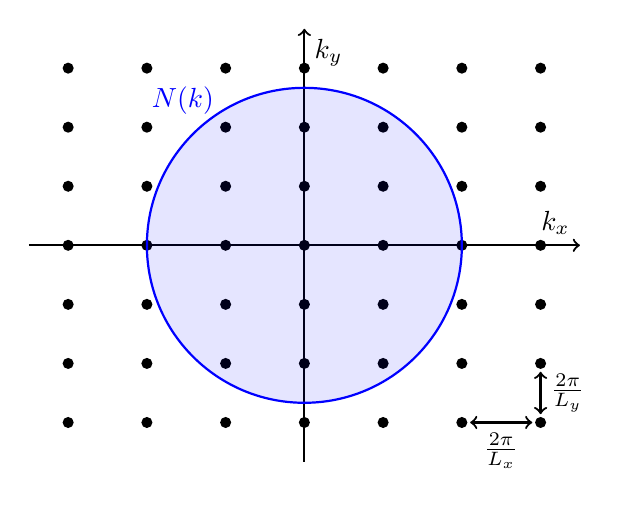
\begin{tikzpicture}[thick]

  % Dot grid
  \def\xrange{3}
  \def\yrange{3}
  \def\ratio{3/4}
  \foreach \x in {-\xrange,...,\xrange}
    {\foreach \y in {-\yrange,...,\yrange}
        {\fill (\x,\ratio*\y) circle[radius=2pt];}}

  % Axes
  \draw[->] (-\xrange-1/2,0) -- (\xrange+1/2,0) node[above left] {$k_x$};
  \draw[->] (0,-\ratio*\yrange-1/2) -- (0,\ratio*\yrange+1/2) node[below right] {$k_y$};

  % Lattice spacing
  \draw[<->,shorten >=3,shorten <=3] (\xrange-1,-\ratio*\yrange) -- (\xrange,-\ratio*\yrange) node[midway,below] {$\frac{2 \pi}{L_x}$};
  \draw[<->,shorten >=3,shorten <=3] (\xrange,-\ratio*\yrange) -- (\xrange,-\ratio*\yrange+\ratio) node[midway,right] {$\frac{2 \pi}{L_y}$};

  % Circle
  \draw[blue,fill=blue,fill opacity=0.1] (0,0) circle (2/3*\yrange);
  \node[blue] at (130:2.4) {$N(k)$};
\end{tikzpicture}

\begin{tikzpicture}[
    g/.style={rectangle,draw,rounded corners,minimum height=6em,inner sep=1em,font=\Huge},
    w/.style={font=\Huge},
    c/.style={node distance=15ex,align=left,font=\huge},
    a/.style={draw,-latex',ultra thick}
  ]

  \node [w,scale=3] (bra) {(};
  \node [node distance=0ex,fill=orange!30,g,right=of bra] (kinetic) {$-\frac{\hbar^2}{2m}\,\vec{\nabla}_{\vec{r}}^2$};
  \node [node distance=2ex,w,right=of kinetic] (plus1) {$+$};
  \node [node distance=2ex,fill=red!30,g,right=of plus1] (external) {$v_\text{ext}(\vec{r})$};
  \node [node distance=2ex,w,right=of external] (plus2) {$+$};
  \node [node distance=2ex,fill=red!30,g,right=of plus2] (hartree) {$v_H(\vec{r})$};
  \node [node distance=2ex,w,right=of hartree] (plus3) {$+$};
  \node [node distance=2ex,fill=red!30,g,right=of plus3] (xc) {$v_{xc}$};
  \node [node distance=0ex,w,right=of xc,scale=3] (ket) {)};
  \node [node distance=0ex,fill=gray!30,g,right=of ket] (phi1) {$\phi_i(\vec{r})$};
  \node [node distance=4ex,w,right=of phi1] (equal) {$=$};
  \node [node distance=4ex,fill=blue!30,g,right=of equal] (energy) {$E_i$};
  \node [node distance=2ex,fill=gray!30,g,right=of energy] (phi2) {$\phi_i(\vec{r})$};

  \node [c,above=of kinetic,xshift=5em] (kinetic comment) {non-rel. Schrödinger equation\\or relativistic Dirac equation};
  \node [c,below=of external,xshift=-10em] (external comment) {crystal ions or\\pseudopotential};
  \node [c,below=of hartree,xshift=5em] (hartree comment) {Poisson equation\\or Hartree potential};
  \node [c,above=of xc,xshift=-11em] (xc comment) {LDA or GGA\\or hybrids};
  \node [c,above=of phi1,xshift=5em] (phi comment) {physical orbitals or not\\mesh density and basis set};
  \node [c,below=of energy] (energy comment) {band structure\\ or not};

  \path [a] (kinetic comment) -- (kinetic.north);
  \path [a] (external comment) -- (external.south);
  \path [a] (hartree comment) -- (hartree.south);
  \path [a] (xc comment) -- (xc.north);
  \path [a] (phi comment) -- (phi1.north);
  \path [a] (phi comment) -- (phi2.north);
  \path [a] (energy comment) -- (energy.south);

\end{tikzpicture}

\begin{tikzpicture}
    \def\gW{2}
    \def\gH{3.2}
    \def\R{0.1}
    \def\boatW{0.3}

    %湖
    \fill[fill opacity=1, draw opacity=1, bottom color=cyan!10!white,  top color=cyan] (\gW, \gH*0.5) coordinate (L) rectangle (\gW+5, 0);
    %岸
    \fill[pattern=north west lines, pattern color=black, ultra thin] (0,0) rectangle (\gW,\gH);
    \draw[very thick] (0,\gH) -- (\gW, \gH);
    \draw[very thick] (\gW,\gH) -- (\gW, 0);
    %滑轮

位置
    \draw[very thick] (\gW,\gH) -- +(45:\R) coordinate (w);

    %滑轮
    \filldraw[very thick, draw=black, fill=black, overlay, remember picture] (w) arc (-135:225:\R);
    %船
    \filldraw[fill=orange] ($(L) + (\R*0.707+\gW+1, \R*0.707)$) coordinate (M) -- ++(-45:\R) -- ++(\boatW,0) -- +(\R*0.707, \R*0.707) -- cycle; 
    %绳子


    \begin{scope}[on background layer]
    \draw[->, blue] ($(w) + (45:\R) + (0,\R)$) coordinate (N) node[above, black]{$O$} -- +(-1.5, 0) node[left]{\large $v$};
    \draw[blue] ($(N) + (0.1, -0.04)$) -- (M) node[midway, right]{$r$};
    \draw[blue] (N) arc (90:50:\R);
    \end{scope}

    %坐标轴


    \draw[->, very thick] (N) -- +(\gW+2, 0) node[right]{$x$};
    \draw[->, very thick] (N) -- +(0, -\gH*0.8-\R) node[below]{$y$};

    %h, x标注
    \draw[-, dashed] (M) -- +(0, \gH*0.5 + \R*1.8) node[midway, right]{$h$};
    \draw[-, dashed] (M) -- +(-\gW-0.9, 0) coordinate (Q) node[midway, above]{$x$};
    %角度标识
    \draw pic[-,"\small $\theta$", thin,angle radius=6,draw=green,angle eccentricity=2.5] {angle = N--M--Q};
\end{tikzpicture}

\begin{tikzpicture}
  \def\R{3}
  \def\ang{45}
  \def\U{2.5}
  \def\X{3}
  \def\Y{3}
  \def\Z{3}
  \def\P{2.5}
  \def\XP{1.5}
  \def\unit{1}
  \coordinate (O) at (0,0) node[left]{$O$};
  \coordinate (X) at ({-\U*sin(\ang)}, {-\U*cos(\ang)}) ;
  \coordinate (Y) at (\Y, 0) ;
  \coordinate (Z) at (0, \Z) ;

  \coordinate (XZ) at ({-\XP*sin(\ang)}, {\P-\XP*cos(\ang)});
  \coordinate (XY) at ({\P-\XP*sin(\ang)}, {-\XP*cos(\ang)});
  \coordinate (YZ) at (\P, \P);

  \coordinate (A) at ({\P - \XP*sin(\ang)}, {\P-\XP*cos(\ang)});

  %坐标轴
  \draw[->, very thick] (O) -- (X) node[left]{$x$};
  \draw[->, very thick] (O) -- (Y) node[right]{$y$};
  \draw[->, very thick] (O) -- (Z) node[above]{$z$};

  %单位矢量


  \draw[->,orange,  very thick] (O) -- ({-\unit*sin(\ang)}, {-\unit*cos(\ang)}) node[left]{$\bm{i}$};
  \draw[->,orange,  very thick] (O) -- (\unit, 0) node[below]{$\bm{j}$};
  \draw[->,orange,  very thick] (O) -- (0, \unit) node[left]{$\bm{k}$};

  %XY平面斜对角线
  \draw[-, dashed, thin, red] (O) -- (XY);

  %方框虚线
  \draw[-, dashed, thin] (A) -- (XZ);
  \draw[-, dashed, thin] (A) -- (YZ);
  \draw[-, dashed, thin] (A) -- (XY);

  \draw[-, dashed, thin] ({-\XP*sin(\ang)}, {-\XP*cos(\ang)}) -- (XZ);
  \draw[-, dashed, thin] ({-\XP*sin(\ang)}, {-\XP*cos(\ang)}) -- (XY);
  \draw[-, dashed, thin] (0, \P) -- (XZ);
  \draw[-, dashed, thin] (0, \P)  -- (YZ);
  \draw[-, dashed, thin] (\P, 0) -- (YZ);
  \draw[-, dashed, thin] (\P, 0) -- (XY);

  %矢量OA
  \draw[->, very thick, blue] (O) -- (A) node[right]{$\bm{r} = x \bm{i} + y \bm{j} + z \bm{k}$} node[midway, above]{$\bm{r}$};

  \fill[red] (A) circle(1.5pt);

  %方位角


  \draw pic[-,"$\alpha$", draw=black,thin,green,angle radius=3,angle eccentricity=2.34] {angle = X--O--A};
  \draw pic[-,"\small$\beta$", draw=black,thin,red, angle radius=8,angle eccentricity=1.54] {angle = Y--O--A};
  \draw pic[-,"$\gamma$", draw=black,thin,purple,angle radius=5,angle eccentricity=2.34] {angle = A--O--Z};
\end{tikzpicture}

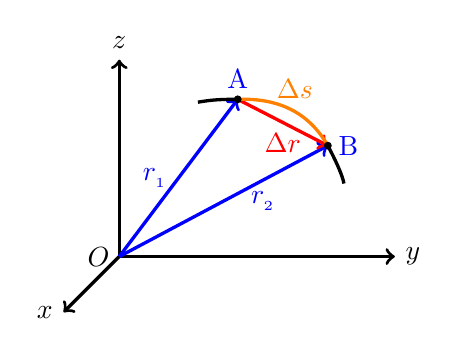
\begin{tikzpicture}
    \def\R{3}
    \def\ang{45}
    \def\U{1}
    \def\Y{3.5}
    \def\Z{2.5}
    \def\P{1.5}
    \def\XP{1.5}
    \def\unit{1}
    \coordinate (O) at (0,0) node[left]{$O$};
    \coordinate (X) at ({-\U*sin(\ang)}, {-\U*cos(\ang)}) ;
    \coordinate (Y) at (\Y, 0) ;
    \coordinate (Z) at (0, \Z) ;

    %坐标轴
    \draw[->, very thick] (O) -- (X) node[left]{$x$};
    \draw[->, very thick] (O) -- (Y) node[right]{$y$};
    \draw[->, very thick] (O) -- (Z) node[above]{$z$};

  \def\ul{0.52}
  \def\angle{28}
  \coordinate (R) at (\angle:\R) ;
  \coordinate (R11) at (\angle:\R - 0.5);
  \coordinate (R2) at (\angle + 25:\R - 0.5) ;
  \coordinate (R1) at (\angle - 10:\R);
  \coordinate (R22) at (\angle + 35:\R - 0.8);

  \draw[->, blue, very thick] (O) -- (R) node[midway,right=6] {$\bm{r}_{_2}$} node[right]{B};

  \draw[->, blue, very thick] (O) -- (R2) node[midway, left] {$\bm{r}_{_1}$} node[above]{A};
  \draw[->, red, very thick] (R2) -- (R) node[midway, below] {$\bm{\Delta r}$};
  \draw[ black, very thick] (R1) to[out=100, in=120](R);
  \draw[ orange,  very thick] (R) to[out=120, in=2] (R2) node[midway, above right = 53]{$\Delta s$};
  \draw[ black,   very thick]  (R2) to[out=180, in=10](R22) ;

\fill[black] (R) circle[radius=0.05];
\fill[black] (R2) circle[radius=0.05];
\end{tikzpicture}

\begin{tikzpicture}[line cap=round]
    \def\R{2}
    \def\X{2.5}
    \def\Y{2.3}
    \coordinate (O) at (0,0) node[below left=-0.2]{$o$};
    \coordinate (X) at (\X, 0);
    \coordinate (Y) at (45:\Y);
    \coordinate (P1) at (30:\R);
    \coordinate (P2) at (60:\R);



    \draw[very thick, ->] (O) -- (X) node[right]{极轴

};
    \draw[very thick, ->, blue] (O) -- (P1) node[right]{$\bm{r_1}$};
    \draw[very thick, ->, red] (O) -- (P2) node[left]{$\bm{r_2}$};

    %角度标识
    \draw pic[-,"$\theta_1$", draw=blue,color=blue, thin,angle radius=6, angle eccentricity=2] {angle = X--O--P1};
    \draw pic[-,"$\theta_2$", draw=red,color=red,thin,angle radius=19, angle eccentricity=1.5] {angle = X--O--P2};
    \draw pic[-,"$\Delta\theta$", draw=green,color=green,thin,angle radius=10, angle eccentricity=1.5] {angle = P1--O--P2};

    \draw[very thick] (O) circle(\R);


    \fill[black] (O) circle(1pt);
    \fill[blue] (P1) circle(1pt);
    \fill[red] (P2) circle(1pt);

    \draw[->, thick] (Y) arc(45:75:\Y) node[left]{$\omega$};
 \end{tikzpicture}

 \begin{tikzpicture}[line cap=round]
  \def\R{3}
  \def\RR{1}
  \def\ang{28}
  \coordinate (O) at (0,0) node[below left]{$O$};
  \coordinate (R) at (\ang:\R);
  \coordinate (etheta) at ({\R*cos(\ang) - \RR*sin(\ang)},{\R*sin(\ang) + \RR*cos(\ang)} );
  \coordinate (er) at ({\R*cos(\ang) + \RR*cos(\ang)},{\R*sin(\ang) + \RR*sin(\ang)} );

  \coordinate (X) at (\R + 0.8,0);
  \draw[->, blue, very thick] (O) -- (R) node[midway,left] {$\bm{r}$} node[below=3, red]{$P(r, \theta)$};
  \draw[->, orange, very thick] (R) -- (etheta) node[above] {$\bm{e_\theta}$};
  \draw[->, orange, very thick] (R) -- (er) node[right] {$\bm{e_r}$};
  \draw[->, very thick, black] (O) -- (X) node[below]{$\text{极轴}$};

  \fill[red] (R) circle[radius=2pt];

 \draw pic[-, "$\theta$", draw=black,thin,red,  angle radius=20,angle eccentricity=1.34] {angle = X--O--R};
  \end{tikzpicture}

  \begin{tikzpicture}[line cap=round]
    \coordinate (O) at (0, 0) node[left]{O};

    \draw[dashed, thin] (O) -- ++(0, -1);
    \draw[thick, gray] (O) ellipse (1 and 0.5);

    \draw[very thick, blue, ->] (O) -- +(0,1.5) node[right]{$\bm{\omega}$};
    % \draw[very thick, orange, ->] (O) -- +(0,1) node[right]{$\bm{\omega}$};

    \draw[very thick, purple, ->] (O) -- (0.6,-0.4) coordinate (A) node[midway, right]{$\bm{r}$};

    \draw[very thick, red, ->] (A) -- +(30:1) coordinate (F) node[right]{$\bm{v} = \bm{\omega} \times \bm{r}$};

    \fill[black] (A) circle(1pt);


    \draw[thin, dashed] (A) -- ++(0.6, -0.4) coordinate (B);

    \draw pic[-,"$\varphi$", thin,angle radius=4,draw=green,angle eccentricity=2.5] {angle = B--A--F};

\end{tikzpicture}
%\end{document}
